\documentclass[a4paper, 11pt]{article}
\usepackage{comment} % enables the use of multi-line comments (\ifx \fi) 
\usepackage{lipsum} %This package just generates Lorem Ipsum filler text. 
\usepackage{fullpage} % changes the margin
\usepackage{graphicx, wrapfig, subcaption, setspace, booktabs}
\usepackage{url}

\begin{document}
%Header-Make sure you update this information!!!!
\noindent
\large\textbf{Exploring delays in air travel in the United States} \hfill \textbf{Sara Arango-Franco} \\
\normalsize \url{github.com/sarangof/air-travel-USA/} 

\section*{Problem Statement}
The RITA \footnote{SIGLA} data set consists on records of airplane trips between airports in the United States since 1987. In this exercise I wondered about flight delays: how do they distribute geographically, how are they related with the relative importance of the most affected airports for domestic air transportation? 

A conversation with an airline schedule specialist made me wonder if it is true that carriers are extending scheduled flight duration in order to have a better on-time performance. 

\section*{Airports as a network}


Explanation: Network representation, etc.


\captionof{table}{Most important airports in terms of betweenness centrality.}
\resizebox{5 cm}{!}{
\centering
\begin{tabular}{|l c|}
\centering
\label{used}
%\hline
\textbf{Airport} & \textbf{ArrDelay} \\
\hline
Atlanta &	0.133890 \\
Dallas 	& 0.085455 \\
Salt Lake City & 	0.084728 \\
Minneapolis  &	0.082088 \\
Anchorage & 	0.058786 \\
Chicago 	& 0.056784 \\
Denver 	& 0.051072 \\
Detroit 	& 0.042831 \\
Houston 	& 0.040318 \\
San Francisco & 	0.038127 \\
%\hline
\end{tabular}
}





\captionof{table}{Worst performing airports in terms of arrival performance:.}
\resizebox{5 cm}{!}{
\centering
\begin{tabular}{|l c|}
\centering
\label{used}
%\hline
\textbf{destin city} & \textbf{ArrDelay} \\
Springfield 	& 63.447158 \\
Aspen 	& 29.995056 \\
Gunnison  &	28.909466 \\
Nantucket &	26.079958 \\
Des Moines &  	24.121120 \\
North Bend 	& 20.736623 \\
Norfolk 	& 20.653845 \\
Chico 	& 19.905077 \\
Eagle 	& 19.462659 \\
Butte 	& 18.991971 \\
%\hline
\end{tabular}
}



\captionof{table}{Worst performing airports in terms of departure performance.}
\resizebox{5 cm}{!}{
\centering
\begin{tabular}{|l c|}
\centering
\label{used}
%\hline
\textbf{origin city} &	\textbf{DepDelay} \\
Champaign &	149.266698 \\
Roanoke 	& 51.956570 \\
Arcata/Eureka & 	48.000720 \\
Klamath Falls &	47.066221 \\
Wichita 	& 39.904703 \\
Appleton &	36.742313 \\
Charlottesville & 	32.597403 \\
Grand Junction & 	31.171125 \\
Fargo 	& 30.783061 \\
Nantucket 	& 29.892045 \\
%\hline
\end{tabular}
}


Arrival vulnerability

\captionof{table}{Most vulnerable airports (arrival).}
\resizebox{5 cm}{!}{
\centering
\begin{tabular}{|l c|}
\centering
\label{used}
%\hline
\textbf{destin city }& \textbf{	ind} 	 \\
Atlanta 	& 0.160344 	 \\
Salt Lake City & 	0.128662 	\\
Minneapolis 	& 0.127824 	 \\
Dallas 	& 0.126783 	 \\
Detroit 	& 0.101268 	 \\
Denver 	& 0.076429 	 \\
Chicago 	& 0.062064 	\\
Houston 	& 0.059642 	\\
Anchorage &	0.057610 \\	
Phoenix 	& 0.055963 	\\

%\hline
\end{tabular}
}








\begin{figure}[!ht]
  \caption{Arrival vulnerability (continental USA).}
  \label{m_days}
  \centering
    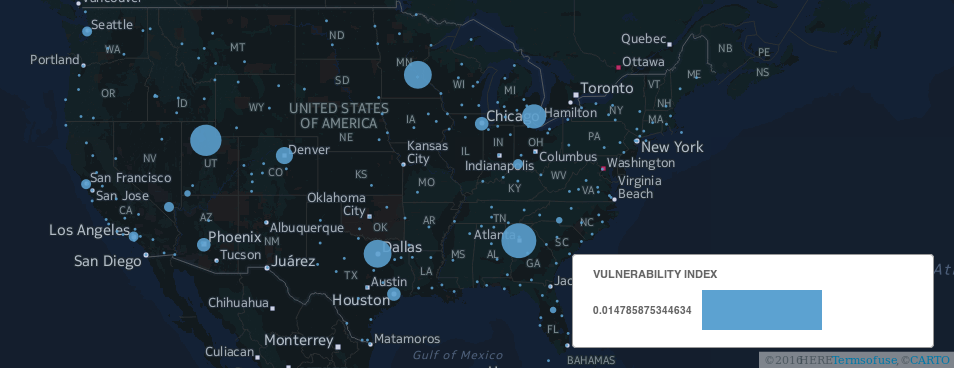
\includegraphics[width=\textwidth]{/home/saf537/Documents/Spotify/air-travel-USA/plots/arrival_vulnerability}
\end{figure}



\captionof{table}{Most vulnerable airports (departure).}
\resizebox{5 cm}{!}{
\centering
\begin{tabular}{|l c|}
\centering
\label{used}
%\hline
\textbf{destin} & \textbf{city 	ind} 	\\
Anchorage & 0.182137 	\\
Atlanta 	& 0.167439 	\\
Salt Lake City & 	0.121132 	\\
Dallas 	& 0.107078 	\\
Minneapolis & 	0.101947 \\	
Chicago 	& 0.084103 	\\
Los Angeles  &	0.083590 \\	
Seattle  &	0.072145 	\\
San Francisco & 	0.065996 	\\
Denver &	 0.062989 	\\

%\hline
\end{tabular}
}



\begin{figure}[!ht]
  \caption{Departure vulnerability (continental USA).}
  \label{m_days}
  \centering
    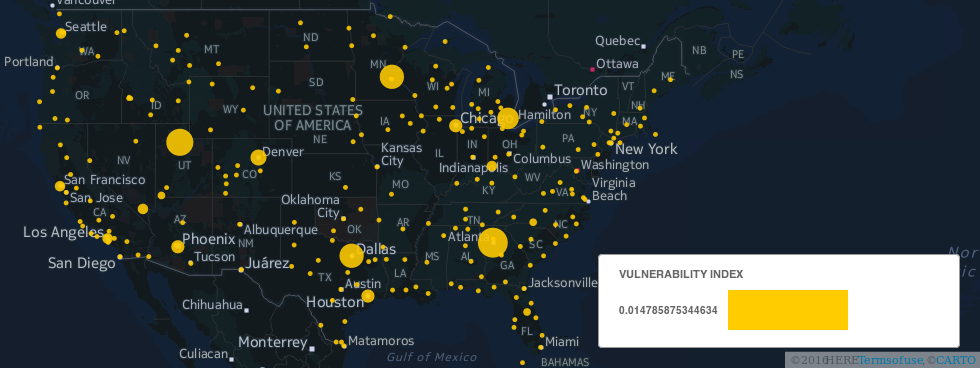
\includegraphics[width=\textwidth]{/home/saf537/Documents/Spotify/air-travel-USA/plots/departure_vulnerability}
\end{figure}


Table: list of most vulnerable airports in terms of arrivals

Table: list of most vulnerable airports in terms of departures

%\begin{figure}[!ht]
%  \caption{Missing days in the dataset.}
%  \label{m_days}
%  \centering
%    \includegraphics[scale=0.6]{/home/saf537/Documents/Spotify/air-travel-USA/plots/test}
%\end{figure}

\section*{Is on-time performance improving with time?}

Explanation of the aggregation that needed to take place: only comparable trips made sense.

plot: scheduling along the years.

plot: total delays along the years.


\begin{figure}[!ht]
  \caption{Scheduled trips length along the years in question.}
  \label{m_days}
  \centering
    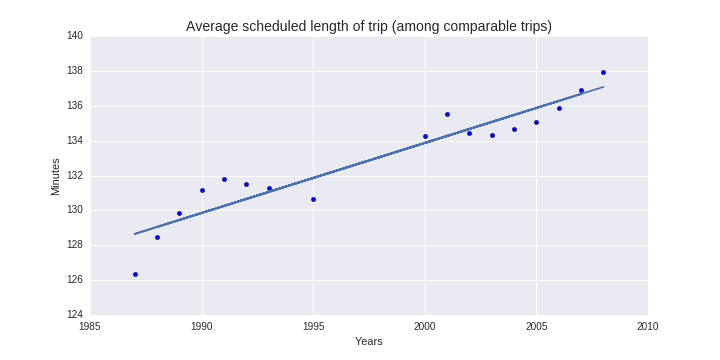
\includegraphics[width=\textwidth]{/home/saf537/Documents/Spotify/air-travel-USA/plots/sch_trips}
\end{figure}


\begin{figure}[!ht]
  \caption{Total delay along the years in question.}
  \label{m_days}
  \centering
    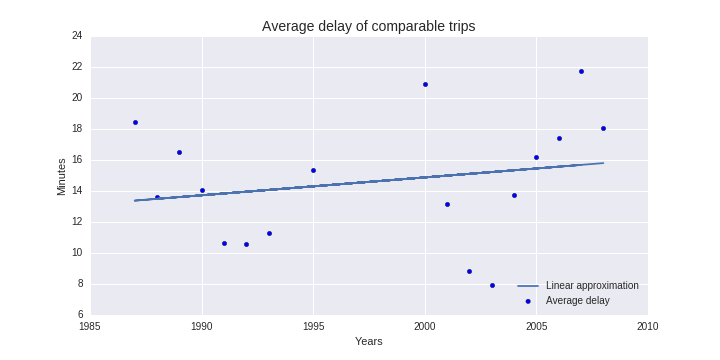
\includegraphics[width=\textwidth]{/home/saf537/Documents/Spotify/air-travel-USA/plots/del_trips}
\end{figure}

\section*{Comments and conclusions}

Clearly this is a biased metric because airports take both national and international flights.

Causality is not proven nor investigated in the last section.

% to comment sections out, use the command \ifx and \fi. Use this technique when writing your pre lab. For example, to comment something out I would do:
%  \ifx
%	\begin{itemize}
%		\item item1
%		\item item2
%	\end{itemize}	
%  \fi




\end{document}
